\documentclass[dvipdfmx]{jsarticle}
\usepackage[final]{graphicx}

% 数式
\usepackage{amsmath,amsfonts}
\usepackage{bm}



\usepackage{listings, jlisting}


\usepackage{xcolor}

%ソースコードの色
\definecolor{commentgreen}{RGB}{0,200,0}
\definecolor{eminence}{RGB}{120,80,250}
\definecolor{weborange}{RGB}{255,165,0}
\definecolor{frenchplum}{RGB}{10,150,200}

\lstset{
        language = {C},
        basicstyle = \ttfamily\small,
        keywordstyle=\color{eminence}\ttfamily\bfseries,
        commentstyle=\color{commentgreen}\textit,
    identifierstyle=\color{black}\ttfamily,
        xleftmargin=.35in,
        frame=lines,
    showstringspaces=false,
        numbers=left,
        stepnumber = 1,
        breaklines=true,
        numberstyle = \ttfamily\normalsize,
    tabsize=4,  
        emph={int, int8_t, int16_t, int32_t, int64_t, uint8_t, uint16_t, uint32_t, uint64_t, char, double, float, unsigned, void, bool},
        emphstyle={\color{blue}}, 
        morekeywords={>, <, ., ;, +, -, *, /, !, =, ~},
        breakindent = 10pt, 
        framexleftmargin=10mm, 
        columns=fixed,
        basewidth=0.5em,
        }

        

\begin{document}

\title{ファイル操作}
\author{古城隆人}
\date{\today}
\maketitle


\newpage
\begin{center}
  \begin{center}
    \Huge ファイル操作とコマンド引数
  \end{center}
\end{center}


\section{課題の内容}
ファイル操作とコマンド引数を理解するために、ファイルの読み書きを行うプログラムを作成する。
\section{プログラムリスト}
\lstinputlisting[caption={main.c}, label={lst:main}]{main.c}

\section{プログラムの説明}
defineを使用して2個のプログラムを一個のプログラムにまとめた。
\subsection{プログラム1個目}

\subsubsection{main関数}
main関数では、表\ref{table:variables}の変数が宣言されています。\\
また、表\ref{table:arguments}の変数をmain関数の引数として受け取ります。\\
以下プログラムの各行ごとの説明を行う。
\begin{itemize}
  \item 14行目のif文でモードの判別を行っている。
  \item 15行目で指定されたファイルが存在するかを確認し、ない場合はNULLとなるため次のif文でtrueとなる。
  \item 20行目のelse文に入るときは引数で指定したファイルが存在しているときである。
  \item 24行目から27行目ではgoto文を用いて標準入力のバッファーが空になるまで繰り返す。
  \item 29行目のwhile文の条件式にてYかNの入力かを確認している。
  \item 30行目でもし、上書きしてはいけない場合はfileを閉じてプログラムをステータス-1で終了する。
  \item 36行目で-iオプションが指定されてないとみなし、引数が1個であることと-iではないことを確認している。
  \item 37行目で指定されたファイルを読み込むためのポインタを取得している。
  \item 38行目から41行目でファイルが存在しない場合はエラーを出力してプログラムを終了する。
  \item 42行目から46行目では引数の入力errorなので、エラーを出力してプログラムを終了する。
  \item 47行目から56行目ではwhile文を使用してファイルに文字の入力をしている。
\end{itemize}



\begin{table}[ht]
  \centering
  \begin{tabular}{|c|c|c|}
    \hline
    型     & 変数名 & 説明                         \\
    \hline
    FILE* & wfp & 書き込み用のファイルのポインタ変数          \\
    char[100] & input & 入力された変数を保持する変数             \\
    int   & ch  & 標準入力で入力された一文字を保持するための変数 \\
    \hline
  \end{tabular}
  \caption{main関数で宣言されている変数のリスト}
  \label{table:variables}
\end{table}

\begin{table}[ht]
  \centering
  \begin{tabular}{|c|c|c|}
    \hline
    型       & 変数名  & 説明                              \\
    \hline
    int     & argc & メイン関数の引数の数                      \\
    char*[] & argv & メイン関数の引数のchar[]型の配列の先頭アドレスのポインタ \\
    \hline
  \end{tabular}
  \caption{main関数で宣言されている変数のリスト}
  \label{table:arguments}
\end{table}

\subsection{プログラム2個目}
\subsubsection{main関数}
main関数では、表\ref{table:variables2}の変数が宣言されています。\\
また、表\ref{table:arguments2}の変数をmain関数の引数として受け取ります。\\
以下プログラムの各行ごとの説明を行う。

\begin{itemize}
  \item 70行目でsrand関数を呼び出し、今の時間のtimestampをseedとして登録している。
  \item 75行目から78行目ではmain関数の引数が2個であることを確認している。引数が2個でない場合はエラーを出力してプログラムを終了する。
  \item 79行目から83行目では引数で指定されたファイルを読み込むためのポインタを取得している。
  \item 84行目ではcount変数に引数で指定された回数を代入している。atoi関数は文字列を数値に変換する関数である。
  \item 85行目から95行目ではfor文を使用してcount回数だけ乱数を生成している。乱数が3桁とも同じ数字である場合はj変数をインクリメントする。また、fprintf関数を使用してファイルに乱数と結果を書き込んでいる。
  \item 96行目では試行回数、あたり回数、期待値、確率をファイルに書き込んでいる。
  \item 99行目ではファイルを閉じてプログラムを終了する。
\end{itemize}


\begin{table}[ht]
  \centering
  \begin{tabular}{|c|c|c|}
    \hline
    型     & 変数名 & 説明                         \\
    \hline
    FILE* & rfp & 書き込み用のファイルのポインタ変数          \\
    int   & ch  & ファイルから読み込んだ文字を保持する変数 \\
    int   & count &  乱数を生成する試行回数\\
    int   & j & 乱数が3桁ともそろった回数を保存する変数\\
    \hline
  \end{tabular}
  \caption{main関数で宣言されている変数のリスト}
  \label{table:variables2}
\end{table}

\begin{table}[ht]
  \centering
  \begin{tabular}{|c|c|c|}
    \hline
    型       & 変数名  & 説明                              \\
    \hline
    int     & argc & メイン関数の引数の数                      \\
    char*[] & argv & メイン関数の引数のchar[]型の配列の先頭アドレスのポインタ \\
    \hline
  \end{tabular}
  \caption{main関数で宣言されている変数のリスト}
  \label{table:arguments2}
\end{table}


\section{結果の説明}
\subsection{プログラム1個目}
\begin{figure}[ht]
  \centering
  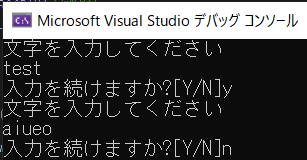
\includegraphics[width=0.5\textwidth]{./img/result_pr1_ndup.png}
  \caption{ファイルが存在しないときの実行結果}
  \label{fig:result_pr1_ndup}
\end{figure}

\begin{figure}[ht]
  \centering
  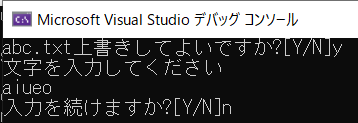
\includegraphics[width=0.5\textwidth]{./img/result_pr1_dup.png}
  \caption{ファイルが存在するときの実行結果}
  \label{fig:result_pr1_dup}
\end{figure}



\section{考察}
\begin{itemize}
  \item ファイルの読み込みに失敗した場合はエラーが出力される。
  \item ファイルの読み込みに成功した場合は、ファイルの内容が標準出力に出力される。
\end{itemize}

\end{document}